\documentclass{article} % For LaTeX2e
\usepackage{nips14submit_e,times}
\usepackage{amsmath}
\usepackage{amsthm}
\usepackage{amssymb}
\usepackage{mathtools}
\usepackage{hyperref}
\usepackage{url}
\usepackage{algorithm}
\usepackage[noend]{algpseudocode}
%\documentstyle[nips14submit_09,times,art10]{article} % For LaTeX 2.09

\usepackage{graphicx}
\usepackage{caption}
\usepackage{subcaption}

\def\eQb#1\eQe{\begin{eqnarray*}#1\end{eqnarray*}}
\def\eQnb#1\eQne{\begin{eqnarray}#1\end{eqnarray}}
\providecommand{\e}[1]{\ensuremath{\times 10^{#1}}}
\providecommand{\pb}[0]{\pagebreak}

\newcommand{\E}{\mathrm{E}}
\newcommand{\Var}{\mathrm{Var}}
\newcommand{\Cov}{\mathrm{Cov}}

\def\Qb#1\Qe{\begin{question}#1\end{question}}
\def\Sb#1\Se{\begin{solution}#1\end{solution}}

\newenvironment{claim}[1]{\par\noindent\underline{Claim:}\space#1}{}
\newtheoremstyle{quest}{\topsep}{\topsep}{}{}{\bfseries}{}{ }{\thmname{#1}\thmnote{ #3}.}
\theoremstyle{quest}
\newtheorem*{definition}{Definition}
\newtheorem*{theorem}{Theorem}
\newtheorem*{lemma}{Lemma}
\newtheorem*{question}{Question}
\newtheorem*{preposition}{Preposition}
\newtheorem*{exercise}{Exercise}
\newtheorem*{challengeproblem}{Challenge Problem}
\newtheorem*{solution}{Solution}
\newtheorem*{remark}{Remark}
\usepackage{verbatimbox}
\usepackage{listings}
\title{Human Genetics: \\
Problem Set I}


\author{
Youngduck Choi \\
CILVR Lab \\
New York University\\
\texttt{yc1104@nyu.edu} \\
}


% The \author macro works with any number of authors. There are two commands
% used to separate the names and addresses of multiple authors: \And and \AND.
%
% Using \And between authors leaves it to \LaTeX{} to determine where to break
% the lines. Using \AND forces a linebreak at that point. So, if \LaTeX{}
% puts 3 of 4 authors names on the first line, and the last on the second
% line, try using \AND instead of \And before the third author name.

\newcommand{\fix}{\marginpar{FIX}}
\newcommand{\new}{\marginpar{NEW}}

\nipsfinalcopy % Uncomment for camera-ready version

\begin{document}


\maketitle

\begin{abstract}
This work contains the solutions to the problem set I
of Human Genetics 2015 course at New York University.
\end{abstract}

\begin{question}[1] 
\end{question}

\smallskip

\begin{solution}
\textbf{a.} As the gamete from the $YY$ pea must be $Y$, the peas in the $F_1$ generation
must contain a $Y$ allele. Since we are given that $YY$ and $Yy$ genotypes result
in yellow color, we have that the peas in the $F_1$ generation must be yellow. In other words,
the expected frequency of yellow peas in the $F_1$ generation of a cross between $YY$ and $yy$
is $1$. \\

\smallskip

\textbf{b.} In part a, we have reasoned that the peas in the $F_1$
generation peas must possess a $Y$ allele. Symmetrically, with the presence of $yy$ parent,
we can conclude that $F_1$ generation peas must possess a $y$ allele. Therefore,
all peas in the $F_1$ generation has $Yy$ genotype. We proceed to compute the expected
frequency of yellow peas in the $F_2$ generation through the Punnett Square analysis with
two $Yy$ parents.

\begin{figure}[h!]
  \caption{A Punnett Square with two $Yy$ parents}
  \centering
    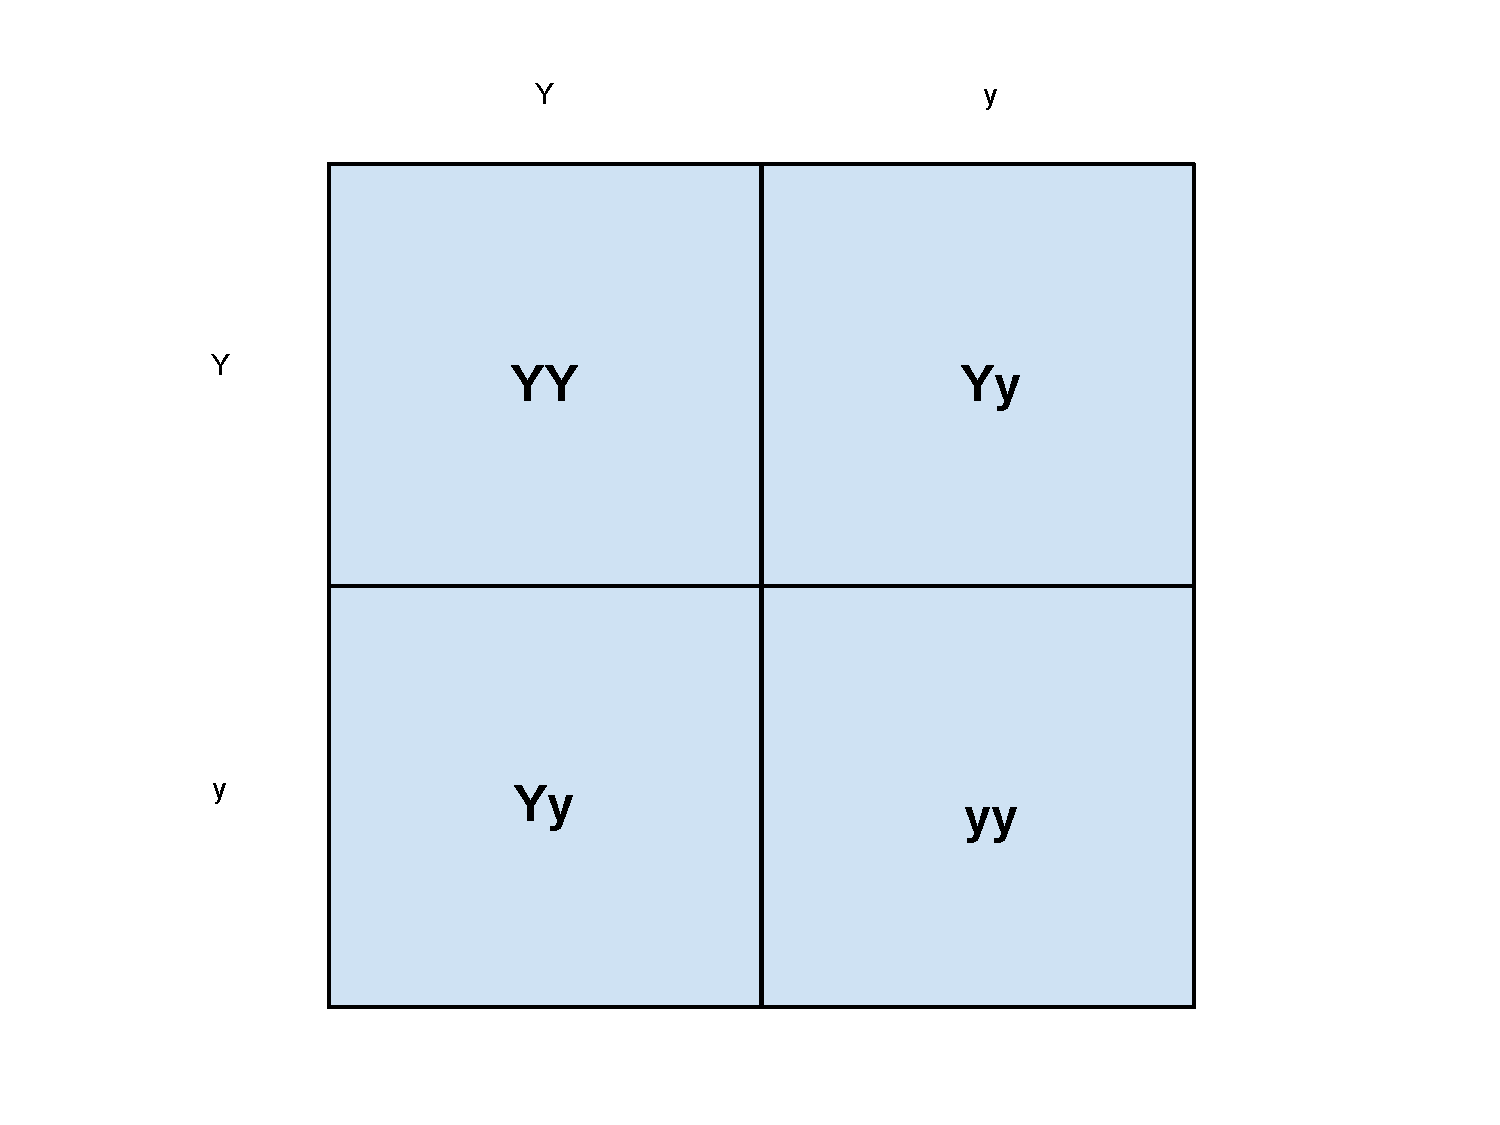
\includegraphics[width=0.8\textwidth]{Punnett.pdf}
\end{figure}

\pagebreak

As the yellow color is the dominant trait, the Punnett Square analysis tells us that
the expected frequency of yellow peas in the $F_2$ generation of the cross is $0.75$. \\

\smallskip

\textbf{c.}
First of all, as the inheritence of $R$ locus and $Y$ locus are independent for peas, 
the extra information about $R$ locus is simply irrelevant. In the previous part,
we computed that the expected frequency 
of yellow peas in the $F_2$ generation of the cross is $0.75$. The expected
frequency of green peas in the $F_2$ generation of the cross is $1 - 0.25$, 
as the sum of the expected freuqnecy of all outcomes must be $1$ and green and yellow
are the only outcomes allowed for color. Hence,
the expected frequency of green peas in the $F_2$ generation of the cross is $0.25$. \\

\smallskip

\end{solution}

\bigskip


\begin{question}[2]
\end{question}
\begin{solution}
We first begin our analysis with a Punnett Square, with two heterozygous parents. \\

\begin{figure}[h!]
  \caption{A Punnett Square with two heterozygous parents}
  \centering
    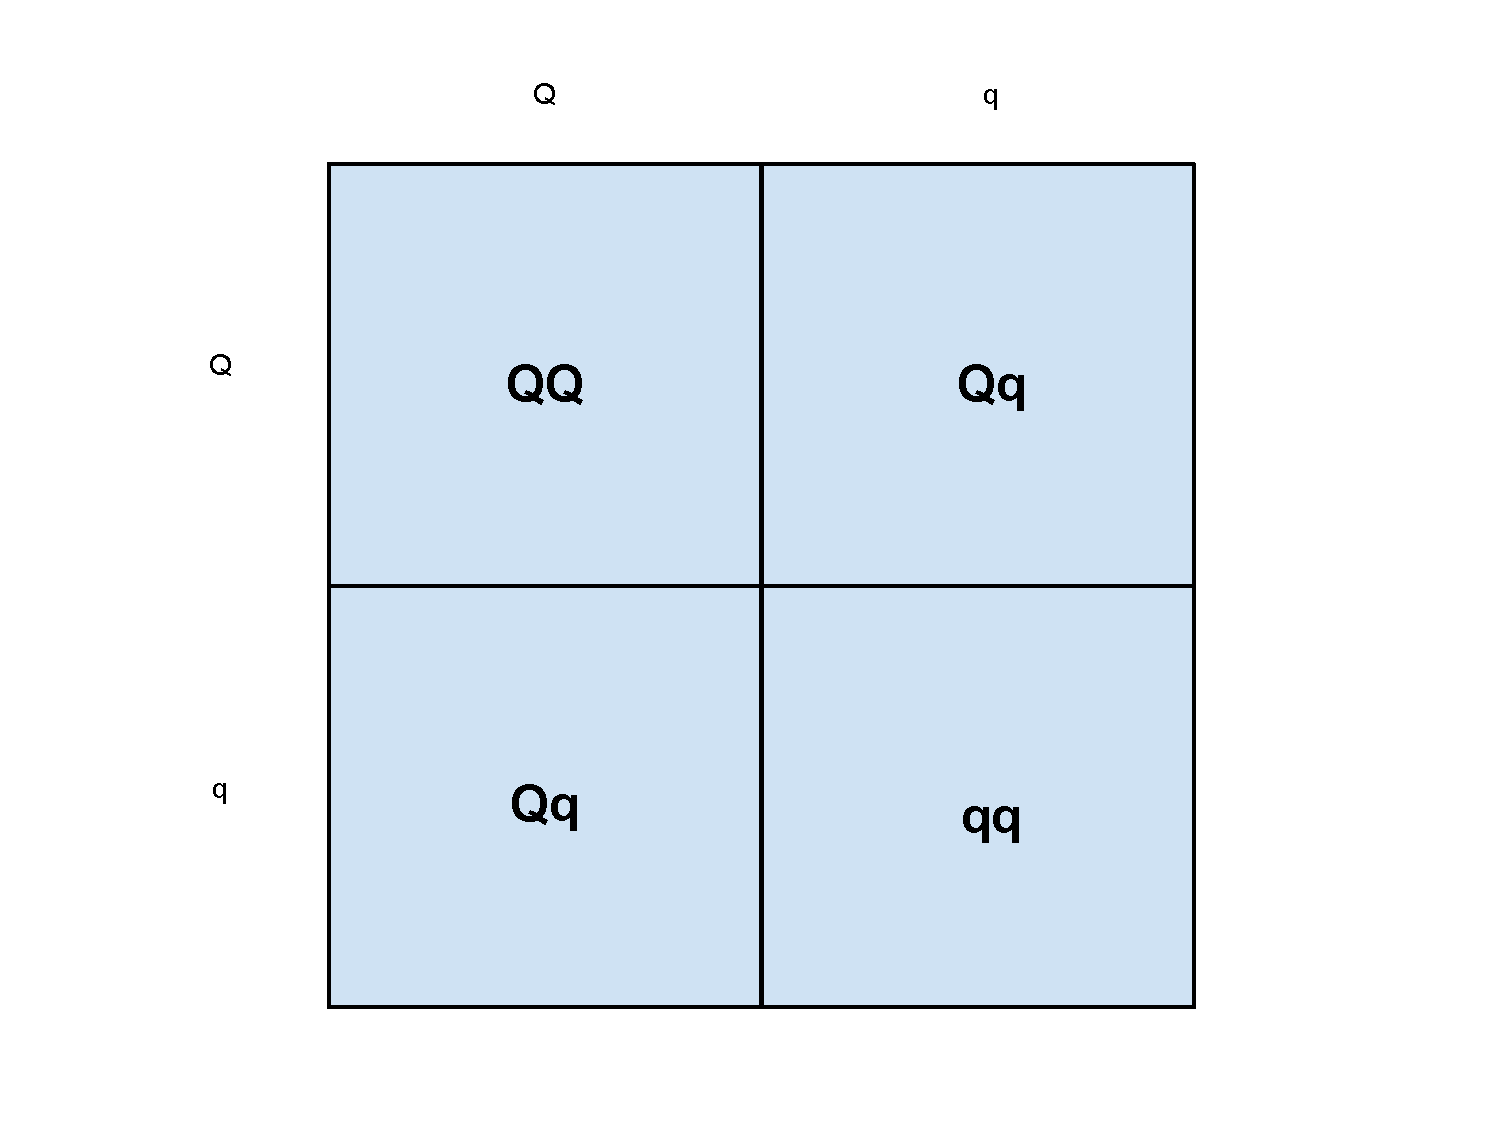
\includegraphics[width=0.8\textwidth]{PunnettII.pdf}
\end{figure}

From the Punnett Square, we observe that the probability of the child having $QQ$ or $qq$ genotype, 
denoted as $P(QQ)$ or $P(qq)$ respecitvely, are both $\dfrac{1}{4}$. There are now two possible cases
that satisfy the given constraint of zero alleles common between the siblings at the locus.
The probability space under consideration can be described as the sample space being
the set of all possible outcomes of birth of two sibilings. The particular set of events, for which 
we wish to compute the probability of is two sibilings having zero alleles in common.
In the first case, the first child has $QQ$ genotype and the second child has $qq$ genotype. As
these events are independent of one another, we obtain that the probability of this case is
$P(QQ)P(qq) = \dfrac{1}{4} \cdot \dfrac{1}{4} = \dfrac{1}{16}$. Now, for the second case the first child 
has $qq$ genotype and the second child has the $QQ$ genotype. As this case is symmetric with the above case,
we have the $\dfrac{1}{16}$ probability again. Hence, the total probability is $\dfrac{1}{16} + 
\dfrac{1}{16} = \dfrac{1}{8}$.
The probability that two siblings, if both of their parents are heterozygous at the locus, will
have zero alleles in common at that locus is $\dfrac{1}{8}$.
\end{solution}

\pagebreak

\begin{question}[3]
\end{question}
\begin{solution}
\textbf{a.} As the father is type $AB$, we know that his genotype is $I^A I^B$. For the case of the mother,
since $O$ is the recessive trait, her genotype is $I^O I^O$. \\

\smallskip

\textbf{b.} The genotype of their children can be either $I^A I^O$ or $I^B I^O$. Since 
$I^A$ and $I^B$ are both dominant to $I^O$, the phenotype of their children can be
either $A$ or $B$. \\

\smallskip

\textbf{c.} Since the father is type $A$, he can have either $I^A I^A$ or $I^A I^O$ 
for his genotype. As the mother is type $B$, she can have either $I^B I^B$ or $I^B I^O$.
We see that the possible genotypes of their children, created through the process of 
segregation, are $I^A I^O$, $I^B I^O$, $I^A I^B$, and $I^O I^O$, which respectively corresponds
to the phenotype $A$, $B$, $AB$ and $O$.
Hence, the possible blood types among their children are $A$, $B$, $AB$, and $O$.


\end{solution}

\bigskip

\begin{question}[4]
\end{question}
\begin{solution}
\textbf{a.} 
Notice that none of the parents possess a $I^B$ allele. As the $AB$ phenotype requires 
a possession of a $I^B$ allele, their first child cannot have the phenotype $AB$ for the
$I$ locus. Hence, the probability that their first child will have the phenotype $AB+$ is
$0$. \\

\smallskip

\textbf{b.} Notice that one parent has $DD$ genotype for the $Rh$ locus. Hence, their first
child will always possess a $D$ allele, which makes the recessive trait $Rh-$ not a
possibility. Therefore, the probability that their first child will have the phenotype $A-$
is $0$. \\

\smallskip

\textbf{c.} The possible genotype for the $I$ locus, in this case, is
$I^A I^A$, and $I^A I^O$, both of which correspond to the phenotype $A$.
Furthermore, the possible genotype for the $Rh$ locus is $DD$ and $Dd$, both of which correspond 
to the phenotype $+$. Therefore, the overall phenotype of their first child is $A+$.
Hence, the probability that their first child will have the phenotype $A+$ is $1$. \\


\end{solution}


\end{document}
